\scanpage{71}

which is probably $=L_i=\operatorname{Ker}(p_i:\mathcal{E}_i\to\Gamma)=$ \unsure{1|the} $\operatorname{Im}(\kappa_i:T(\overline{K})\to\mathcal{E}_i\cap\pi)$.
Thus we find that \deleted{\unsure{$f$}} the \deleted{homomorphism} $\pi$-conjugacy class of groups over $\Gamma$ of $f:\mathcal{E}'\to\mathcal{E}$ suffices to determine the homomorphism $\mathcal{D}'\to\mathcal{D}$ in the messy category.
I presume that a little sweat would make it possible to prove that this still works in the general case (without assuming the $\Gamma_i=\operatorname{Im}(\unsure{\mathcal{E}_i}\to\Gamma)$ equal to $\Gamma$).
This means (in the present case) that the essential structure which describes $(X,S)$ is that of an \deleted{\illegible{1}} ``\uline{outer extension}'' of $\Gamma$ by a group $\pi$ [surjective outer homomorphism from a group, with kernel a $\pi$], with $\pi$ equipped with a \uline{loop structure} i.e. \deleted{conjugacy class} \inserted{of homomorphisms} \uline{outer}
\[
\kappa_i:T\,\unsure{\text{\deleted{\illegible{1}}}|\mu}\,(=T(\overline{K})\,\unsure{\text{\deleted{)}}}\,\overset{\text{noncanonically}^{t}}{\simeq}\,\widehat{\mathbf{Z}})\to\pi
\]
(satisfying certain conditions), the

\margin{70}

\scanpage{72}
\mspage{34}

homomorphisms \inserted{from} $\mathcal{E}'\to\Gamma$ (kernel $\pi'$) into $\mathcal{E}\to\Gamma$ (kernel $\pi$) being the $\pi$-conjugacy classes of homomorphisms $\mathcal{E}'\to\mathcal{E}$ of groups over $\Gamma$, inducing homomorphisms $\pi'\to\pi$ compatible with the loop structure.

9. Tangential structure at the $s\in S$.
\margin{[The sections of extensions ``of the second type'']}

Returning to the \inserted{``intrinsic''} description of the $(X,S)$ by
$\Pi_{D^*}\to\Pi_U\to\Pi_e$, an $s_i\in S$ thus corresponds to a connected component \inserted{$\Pi_{D_i^*}$} of $\Pi_{D^*}$, or \inserted{a $\Pi_{D_i}$} of its quotient $\Pi_D$ --- consider
\[
\Pi_{D_i^*}\xrightarrow{\unsure{\sigma_i=\Pi_{f_{D_i^*D_i}}|\sigma_i=\sigma_{D_i^*D_i}}}\Pi_{D_i}.
\]
We are going to describe certain sections (up to isomorphism) of this \deleted{\unsure{functor}} \inserted{morphism} of groupoids, i.e. \inserted{pairs $(\gamma,\lambda)$} functors
$\Pi_{D_i}\xrightarrow{\gamma}\Pi_{D_i^*}$ and an isomorphism $\sigma_i\circ\gamma\overset{\lambda}{\simeq}\operatorname{id}$.
If we choose a $\widetilde{D}_i^*\in\operatorname{Ob}\Pi_{D_i^*}$ (universal covering of $D_i^*$), whence a \inserted{surjective} homomorphism
\[
\mathcal{E}_i=\operatorname{Aut}(\widetilde{D}_i^*)\to\Gamma_i
=\operatorname{Aut}(\sigma_i(\widetilde{D}_i^*)=\widetilde{D}_i),
\]
\unsure{the} \deleted{datum} datum of $(\gamma,\unsure{\lambda_i|\lambda})$, \inserted{and of an isomorphism $\gamma(\widetilde{D}_i)\simeq\widetilde{D}_i^*$ giving the identity isomorphism on applying the $\sigma_i$,} amounts to that of a homomorphism $\Gamma_i\to\mathcal{E}_i$.
--- and the isomorphism classes of the pairs $(\gamma,\lambda)$ correspond to the \inserted{$L_i$}-conjugacy classes

\margin{71}

\scanpage{73}

($L_i=\operatorname{Ker}(\text{\deleted{\illegible{1}}\inserted{$\mathcal{E}$}}_i\to\Gamma_i)$) of \deleted{morphisms} \inserted{sections} of the extension $\mathcal{E}_i$ of $\Gamma_i$ by $L_i$.

This being so, \unsure{we have}
\[
\Gamma_i=\operatorname{Gal}(\overline{K}_i/K_i).
\]
where $K_i=k(s_i)$, $\overline{K}_i$ is the algebraic closure of $K_i$ defined by $\widetilde{D}_i$ (a priori, it is not \unsure{canonical\textsuperscript{ly}} isomorphic to $\overline{K}$ over $K$\ldots), and the classes of \deleted{\unsure{extensions}} \inserted{splittings} of extensions form a \uline{torsor} \inserted{$\Sigma_i$} (if there are any, and we know that there are\ldots) under $H^1(\Gamma_i,L_i)$, or again, since $\kappa_i:L_i\xleftarrow{\sim}T(\overline{K}_i)$, under
\[
H^1(\operatorname{Gal}(\overline{K}_i/K_i),T(\overline{K}_i))
\simeq H^1(K_i,\unsure{T_e|T_\ell}(G_m))
\simeq\varprojlim_n H^1(K_i,\mu_n).
\]
Now the Kummer exact sequence gives
\diagram{\begin{tikzcd}[ampersand replacement=\&,column sep=small]
0 \arrow[r] \& H^0(K_i,\text{\deleted{\unsure{$\overline{K}$}}}\,G_m)_n \arrow[r] \arrow[d,equal] \& H^1(K_i,\mu_n) \arrow[r] \& {}_nH^1(K_i,G_m) \arrow[r] \arrow[d,equal] \& 0 \\
\& (K_i^*)_n \&\& 0 \&
\end{tikzcd}}
i.e. $H^1(K_i,\mu_n)\simeq(K_i^*)_n$, hence
\[
H^1(K_i,T(G_m))\simeq\varprojlim_n(K_i^*)_n
\]

\margin{72}

\scanpage{74}
\mspage{35}

Note that we have a Kummer homomorphism
\[
K_i^*\to\underbrace{H^1(K_i,T(G_m))}_{\mathcal{H}_i}
\simeq\varprojlim(K_i^*{}_n)
\]
whose kernel consists of the $\unsure{x}\in K_i^*$ such that for $\forall\ n\in\mathbf{N}$, we have $x\in K_i^{*n}$.
Since $K_i$ is of finite type over $\mathbf{Q}$, this homomorphism is injective, i.e. $K_i^*$ is identified with a subgroup of $\mathcal{H}_i$.

This being so, \unsure{we are going to} define, in the torsor $\Sigma_i$ under $\mathcal{H}_i$ of splittings of $D_i^*$ over $D_i$, a sub-\inserted{$K_i^*$}-torsor (i.e. an element of $\Sigma_i/K_i^*$).
For this,

\deleted{note that $\mathcal{O}_{s_i}=\widehat{\mathcal{O}}_{X,s_i}$ canonically contains the subfield $K_i$ (for example as the integral closure of $K$ in $\mathcal{O}_{s_i}$), and that the choice of a uniformizer $t$ of $\mathcal{O}_{s_i}$ defines a \deleted{subfield} \inserted{$K_i$-}\deleted{$K[[t$} isomorphism $\mathcal{O}_{s_i}\simeq K_i[[T]]$, (by the condition $T\mapsto t$). Note that we have}

\margin{73}

\scanpage{75}

\deleted{(with $\widetilde{D}_i^*$) an algebraic closure \inserted{$\overline{K}_s$} of $K_s$ (fraction field of $\mathcal{O}_s$), defining \deleted{\unsure{just} \illegible{1}} \inserted{an} algebraic closure $\unsure{\overline{K}_i}$ of $K_i=k(s)$, \unsure{which is} precisely $\overline{K}_i$. \deleted{This being so, in $\overline{K}_s$ the subfield}}
\margin{make a general local argument, dropping the index \unsure{$i$}.}

Let us consider more generally the case of a field $k$ $(=K_i)$ of characteristic $0$, and of a \deleted{\illegible{1}} $k$-algebra $\mathcal{O}$ which is a henselian \inserted{gauge} with residue field $k$.
\inserted{let $L$ be the fraction field of $\mathcal{O}$}
We are going, for \unsure{ever\textsuperscript{y}} uniformizer $t$ of $\mathcal{O}$, to define a section $(\gamma,\lambda)$ \unsure{of the|of the} \deleted{\unsure{$\Pi_K$}} \deleted{\unsure{the category}} \unsure{groupoid|groupoids} of algebraic closures of $L$, to that of universal coverings of $\unsure{\operatorname{Spec}(\mathcal{O})|\operatorname{f\acute{e}t}(\mathcal{O})}$ or, what amounts to the same thing, of algebraic closures of $k$. For this,

let
\[
\mathcal{O}(n,\unsure{t|s})=\mathcal{O}[T_n]/(T_n^n-s),\quad\text{and}
\]
\[
\mathcal{O}(\infty,t)=\varinjlim_n\mathcal{O}(n,t),\quad
\text{by }T_{n\,\unsure{t|s}}\mapsto T_{mn\,\unsure{t|s}}^{\,m}.
\]
\deleted{then $\mathcal{O}(\infty,t)$ is \unsure{again a} henselian gauge}
\deleted{\unsure{Put}}
$L(n,t)=\mathcal{O}(n,t)\otimes_{\mathcal{O}}K=$ fraction field of $\mathcal{O}(n,t)$, $L(\infty,t)=\varinjlim_n L(n,t)$ the fraction field of $\mathcal{O}(\infty,t)$. This is

\margin{74}

\scanpage{76}
\mspage{36}

an algebraic extension of $L$, and for \unsure{ever\textsuperscript{y}} \deleted{algebraic closure $\overline{k}$ of $k$, \illegible{1} $L\otimes_k\overline{k}$ is algebraically closed} \inserted{finite, or ind-finite extension} $k'$ of $k$, putting $\mathcal{O}'=\mathcal{O}\otimes_k k'$ (which is also a henselian gauge over $k'$ with residue field $k'$, with fraction field $L'\simeq L\otimes_k k'$), we have \inserted{canonical isomorphisms} \deleted{\illegible{1}}
\[
\mathcal{O}(\unsure{n|\infty},t)\otimes_{\mathcal{O}}\mathcal{O}'\simeq\mathcal{O}'(\unsure{n|\infty},t)
\]
\[
\mathcal{O}(\infty,t)\otimes_{\mathcal{O}}\mathcal{O}'\simeq\mathcal{O}'(\infty,t)
\]
whence
\[
L(\unsure{n|\infty},t)\otimes_k\unsure{\overline{k}'|k'}\simeq L'(\unsure{n|\infty},t)
\]
\[
L(\infty,t)\otimes_k k'\simeq L'(\infty,t)
\]
Now if $\unsure{k'|\overline{k}'}$ is algebraically closed, \deleted{we know that} $\mathcal{O}'$ strictly henselian, we know that $L'(\infty,t)$ is then algebraically closed.
Besides \deleted{\illegible{1}} since $\unsure{\overline{k}'|k'}\subset\mathcal{O}'(\infty,t)\subset L'(\infty,t)$, in this case \unsure{$k$} $k'$ \deleted{\illegible{1}} is identified with the algebraic closure \inserted{$\overline{k}$} of $k$ in $L'(\infty,t)=\overline{L}$.
So we have indeed found a section of $\Pi_{D^*}$ over $\Pi_D$.

But if we replace $s$ by $s'=su^n$, with $u\in\mathcal{O}^*$, we find isomorphisms
\diagram{$\unsure{\lambda(n,u)}:\quad$\begin{tikzcd}[ampersand replacement=\&,column sep=large]
\mathcal{O}(n,s) \arrow[r] \arrow[d,equal] \& \mathcal{O}(n,s') \arrow[d,equal] \\
\mathcal{O}[T_n]/(T_n^n-s) \& \mathcal{O}[T_n]/(T_n^n-s')
\end{tikzcd}}
by $T_n\to uT_n$
whence by passing to the limit
\[
\lambda(\infty,\unsure{u|n}):\mathcal{O}(\infty,s)\unsure{\longrightarrow}\mathcal{O}(\infty,s')
\]
inducing $L(\infty,s)\xrightarrow{\sim}L(\infty,s')$ an isomorphism of extensions \inserted{of $L$}

\margin{75}

\scanpage{77}

whence an isomorphism between the corresponding sections of the $\Pi_{L}$ over $\Pi_k$.
This implies that if $s,s'$ differ by a $\unsure{u|v}\in\mathcal{O}^*$ such that its image in $k$ is $1$ \deleted{(so $\unsure{u|v}\in$ \illegible{2}} \inserted{i.e. $\unsure{u|v}\in1+m$} (which is a divisible subgroup of $\mathcal{O}^*$] then $s,s'$ define isomorphic sections.
Thus we find a canonical map
\[
\begin{array}{ccl}
(m/m^2)^* & \to &
\begin{gathered}
\text{isomorphism classes of sections of}\\
\Pi_L\text{ over }\Pi_k\quad\text{i.e. of}\\
\operatorname{Gal}(\overline{K}/L)\to\operatorname{Gal}(\overline{k}/k)
\end{gathered}
\\[1ex]
\begin{gathered}
\deleted{\unsure{\text{(and}}}\text{(set of}\\
\text{bases of }m/m^2\text{)}\\
\text{which is a}\\
\text{torsor under}\\ k^*
\end{gathered}
&&
\begin{gathered}
\text{(which is a torsor under}\\
H^1(\operatorname{Gal}(\overline{k}/k),T(\overline{k}))\\
\text{i.e. under }H^1(k,T(G_m))\ldots)
\end{gathered}
\end{array}
\]

We see at once that this map is compatible with the homomorphism
\[
\Theta:k^*\to H^1(k,T(G_m))
\]
on the groups acting on these torsors.
In the case where this homomorphism is injective (for example $k$ \deleted{we thus find an \unsure{embedding}} of finite type over $\mathbf{Q}$) we thus find an embedding of $m/m^2$ as a sub $\Theta(k^*)$-torsor of the $H^1(k,T(G_m))$-torsor

\margin{76}

\scanpage{78}
\mspage{37}

of splittings of $\Pi_{D^*}$ \inserted{($\simeq$ groupoid of algebraic closures of $L$)} over $\Pi_D$ ($\simeq$ groupoid of algebraic closures of $\unsure{k}$).

Returning to the case of the \deleted{\illegible{1}} $\Pi_{D^*}\to\Pi_U\to\Pi_e$ $\unsure{\kappa|K}\ldots$, and of the \deleted{\illegible{1}}
\[
\mathcal{D}:T(\overline{K}^*)\xrightarrow{\kappa_i}\mathcal{E}_i\hookrightarrow\mathcal{E}\xrightarrow{p}\Gamma
\]
which make them explicit, we thus find an additional structure on $\mathcal{E}$ or $\mathcal{D}$ via \deleted{\unsure{on}} the extensions $\mathcal{E}_i$ of $\Gamma_i\subset\Gamma$ by $T(\overline{K}^*)$, namely \deleted{\unsure{some}} \inserted{$\forall i\in I$} sub-$K_i^*$-torsor\unsure{s} in the torsor under
$H^1(K_i,T(G_m))\simeq\varprojlim(K_i^*)_n$ of \inserted{classes of} splittings of $\mathcal{E}_i$.
We ought to make explicit the behavior of this additional structure with respect to morphisms (coming from geometric situations) and the relation with the norm of differential $1$-forms --- I'm too lazy to make it explicit at length and in detail!

The new thing I retain above all is that for $I\ne\varnothing$ and the $\mathcal{E}_i\to\Gamma$ surjective (to simplify), we find \inserted{$\forall i$} \unsure{a|some} ``\unsure{transcendental|transcendental} \unsure{family|families}'' of splittings of $\mathcal{E}\to\Gamma$ (via splittings of $\mathcal{E}_i$ over $\Gamma$) --- \unsure{essential\textsuperscript{ly}} \unsure{indexed}

\margin{77}

\scanpage{79}

by $H^1(\unsure{K_i|K},T(G_m))\simeq\varprojlim(K^*)_n$ (more precisely, by a torsor under the aforesaid)

--- in this family, a subfamily of splittings which one can call ``geometric'', indexed by $K^*$ (more precisely, a subtorsor\ldots).
We check that the \inserted{classes of $\pi$-}splittings obtained \unsure{for|by} distinct indices $i,i'$ are distinct, even on reducing to the corresponding \unsure{$\pi$-}splittings of the extension of $\Gamma$ by $\pi_{\mathrm{ab}}$ deduced from the extension $\mathcal{E}$ of $\Gamma$ by $\pi$ (I am not going into the details of the verifications, via Mordell-Weil\ldots) and distinct from the splittings associated with the rational points$/K$ of $X\backslash S$.

\margin{\figure{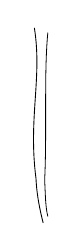
\begin{tikzpicture}[x=1cm,y=1cm,line cap=round]
\draw[line width=.32pt] (0,0) .. controls (.10,-.64) and (-.08,-1.14) .. (.02,-1.91)
 .. controls (.03,-2.14) and (.08,-2.35) .. (.11,-2.47);
\draw[line width=.29pt] (.17,-.06) .. controls (.12,-.59) and (.16,-1.31) .. (.13,-1.93)
 .. controls (.14,-2.13) and (.14,-2.27) .. (.17,-2.39);
\end{tikzpicture}}}
We ought to correct the messy conjecture in the case (\uline{$\overline{\mathrm{III}}$}), by stating (with all reservations, again!) that there are (perhaps) no other splittings of the extension $\mathcal{E}$ of $\Gamma$ by $\pi$ than those ....

\margin{78}

\scanpage{80}
\mspage{38}

10. Adjustment of the hypotheses (remorse).

I realize that in the definition of the morphisms $(X',S')\xrightarrow{f}(X,S)$, the hypothesis $f^{-1}(S)_{\mathrm{red}}=S'$ is too narrow --- we must take \uline{arbitrary} morphisms $f:X'\backslash S'\to X\backslash S$ (extending of course to $\widehat{f}:X'\to X$).
We will thus have $S'\supset\widehat{f}^{-1}(S)_{\mathrm{red}}$, but $S'$ may be strictly larger than $\widehat{f}^{-1}(S)_{\mathrm{red}}$.
We must then adjust the description of the ``messy category'' accordingly --- the objects remain the diagrams of groupoids
\[
\mathcal{D}:\Pi_{D^*}\to\Pi_U\to\Pi_e
\]
(plus Kummer datum) but a morphism $f$ from a $\mathcal{D}'$ into a $\mathcal{D}$ no longer necessarily defines a $\Pi'_{D^*}\to\Pi_{D^*}$ (in addition to $\Pi'_U\to\Pi_U$) one must specify a subset $I'_f$ of $I'=\pi_0(\Pi'_{D^*})$, and specify only
\[
\Pi'_{D^*,I'_f}\xrightarrow{f_{D^*}}\Pi_{D^*}
\]
(with commutation datum \inserted{$\unsure{\alpha_{D^*U}}$} relative to the square with $f_U$).
Of course, in the description in terms of $\mathcal{E}',\mathcal{E}$ etc., we require that for $i'\in I'\backslash I'_f$, $f_{\mathcal{E}}:\mathcal{E}'\to\mathcal{E}$ is trivial on $\mathcal{E}'_{i'}\subset\mathcal{E}'$ --- and $\tau$ is defined as $I'_f\to I$ ; \unsure{some|the} data relating to the $i'\in$

\margin{79}
